\fancychapter{\ac{TEE} replication using the \ac{RR} model}\label{chap:tee}
\cleardoublepage{}

As we have discussed previously, \acp{TEE} are an interesting
option deploying replicated systems in an untrusted public cloud.
In this chapter, we present the \acf{TEEMS}, a replicated metadata
service for trusted cloud storage. \ac{TEEMS} has a double purpose in
the context of this dissertation: it showcases a practical system
using the \ac{RR} fault model and associated register and
\ac{SMR} protocols and provides the means of enhancing existing
cloud storage systems such that they can be trusted and remotely
attested in the same fault model as \acp{TEE} (and, by extension,
used by them as a persistent storage, with rollback protection).

This chapter is organized as follows.
Section~\ref{sec:teems_design}
provides the motivation and design of \ac{TEEMS}, followed by
Section~\ref{sec:teems_impl}, which describes the implementation
of \ac{TEEMS}. Finally, Section~\ref{sec:teems_eval} presents an
extensive evaluation of \ac{TEEMS} using real-world workloads
across different deployments.

\section{\ac{TEEMS}: Metadata service for trusted cloud
storage}\label{sec:teems_design}


\subsection{Motivation}

\acp{TEE} have enabled services like Azure Confidential
Computing~\cite{azure-conf} and Google Confidential
VMs~\cite{google-confVM}, where Cloud tenants can use compute
services without trusting the platform provider.  However, the
strong security properties from \acp{TEE} do not automatically
extend to cloud storage. \new{To create a cloud-based system with
similar strong security guarantees of \acp{TEE}, it is only
natural to consider using \acp{TEE} as its building blocks.} A
\ac{TEE}-encapsulated metadata service, replicated for
availability and fault-tolerance, can maintain encryption keys
and version information for data blobs stored in untrusted Cloud
storage.  By ensuring confidentiality, integrity, and freshness
of the metadata, the service extends the same guarantees to the
encrypted and versioned data blobs. Moreover, by supporting an
atomic update operation on metadata, the service enables
concurrent sharing of data blobs.

\new{This approach needs to be integrated at the replication
level. Fundamentally, even assuming an efficient way for
storing the state of a single \ac{TEE}, this solution would still be
unable to support concurrent sharing between multiple \acp{TEE}. This
is because ensuring freshness of a single \ac{TEE}'s own state relies
on persistently storing a monotonic counter~\cite{ariadne,rote,ice}
or a top-level hash~\cite{memoir}, which can only be updated by
the \ac{TEE} itself.  Concurrent sharing of persistent state instead
requires atomic, concurrent updates of state blobs and their
associated metadata (e.g., counter).
}

We designed and implemented a replicated metadata service called
\ac{TEEMS} (for \ac{TEE}-based Metadata Service) based on the
\ac{RR} fault model. \ac{TEEMS}'s replicas can be hosted in a
diverse set of cloud providers for high availability and
resilience.
%
\ac{TEEMS} provides a read/write interface for metadata and guarantees that
readers always receive the metadata (e.g., encryption key) of the most
recent version of a data blob.  \ac{TEEMS} also supports access control
policies for metadata, and therefore allows clients to selectively
share the associated data blobs.  The service therefore enables
trusted storage services that extend the strong guarantees of today's
\ac{TEE}-based cloud compute services to persistent storage.

\subsection{\ac{TEE}-grade cloud storage with \ac{TEEMS}}

Clients can use \ac{TEEMS} to lend untrusted cloud storage \ac{TEE}-level
guarantees, by using the API in Table~\ref{tab:teems}.
\ac{TEEMS} maintains metadata for each data blob, i.e. a short summary of
the most recent version of a data blob, namely its hash and encryption
key. The encrypted data blob is then stored in an ordinary cloud
storage service. This extends the integrity, confidentiality,
freshness and selective concurrent sharing properties of the
metadata service to the cloud storage, while relying on the cloud
service only for storage and availability.

\begin{table}[!t]
    \centering
    \renewcommand{\arraystretch}{0.9} % this reduces the vertical spacing between rows
    \begin{small}
    \begin{tabular}{rll}
        \hline
        Return Value && {Command and Arguments}\\
        \hline
        \{\lArg{status}\} &\eq& {\sysC{teems-init}(\lArg{client ID})}\\
        \{\lArg{status}\} &\eq&{\sysC{teems-close}}()\\
        \{\lArg{status}\} &\eq&{\sysC{teems-write}}(\lArg{id}, \nArg{val})\\
        \{\lArg{status}, \nArg{val}, \lArg{ver}\} &\eq&{\sysC{teem-read}}(\lArg{id})\\
        \{\lArg{status}\} &\eq&{\sysC{teems-delete}}(\lArg{id})\\
        \{\lArg{status}\} &\eq&{\sysC{teems-change-policy}}(\lArg{id}, \lArg{policy-code})\\
        \hline
    \end{tabular}
    \end{small}
    \caption{\ac{TEEMS} Interface}\label{tab:teems}
\end{table}

Concurrent sharing of mutable data fundamentally requires a
read-modify-write operation (i.e., some form of \ac{SMR}).
However, state machine operations are more expensive than
read/write register operations. \ac{TEEMS} minimizes the use of
state machine operations in situations where writers typically
perform multiple updates of a data blob before other writers
perform an update as follows.  We mediate access to the metadata
via single writer policies, and implement policy changes via the
more expensive read-modify-write state machine operation. Simply
reading and updating the metadata of a blob (by the current
writer) is implemented using efficient distributed register
operations.  This approach ensures safe concurrent sharing of
data blobs while minimizing the more expensive policy changes to
cases when the writer for a blob changes. The full \ac{TEEMS}
interface is summarized in Table~\ref{tab:teems}.

Storage operations involve the following sequence of steps.  When an
operation to write a new data blob $d$ associated with id $i$ is
invoked, the client library starts by generating a symmetric
encryption key $k$. In our implementation, we use an authenticated
encryption scheme (AES-GCM), which generates a ciphertext ($\langle d
\rangle_k$) and a MAC ($MAC(d)$) of $d$.
%
The encrypted object and corresponding MAC are then stored in one
or more untrusted cloud storage services, under a randomly
created identifier $i_{store}$. Let $a$ be the access control
list for the newly stored data blob $d$. After the data has been
successfully written to untrusted storage, the library contacts
the \ac{TEEMS} metadata service to update the metadata for id $i$:
\[ \langle i,k,a,i_{store},MAC(d) \rangle   \]
%
The write operation concludes successfully after both the data
write and the metadata update complete. Finally, the library
deletes earlier versions of the blob from the data store.

When a read for id $i$ is invoked, the client library starts by
querying the \ac{TEEMS} service for the most recent version of
the metadata associated with the id $i$. After retrieving the
tuple $\langle i,k_i,i_{store},MAC(d_i) \rangle$, the client
library then uses the id $i_{store}$ to retrieve the encrypted
data from untrusted storage. This encrypted data $\langle
d'\rangle_{k_i}$ is read and then decrypted using $k_i$,
obtaining $d'$ and $MAC(d')$. Finally, its integrity  is
validated by comparing $MAC(d')$ and $MAC(d_i)$.

Finally, the access to the untrusted storage can be optimized by
employing caching at the client. We can either cache full blobs (to
avoid having to access the untrusted store) or name hints (for
enabling parallel access to the metadata service and the untrusted
store).  In either case, the metadata always has to be fetched and
compared with the cached or retrieved version, since only the
\ac{TEEMS} metadata service can ensure freshness of data blobs.

\subsection{Leveraging different storage protocols}

\ac{TEEMS} implements the metadata read/write operations efficiently using
our \ac{RR}-tolerant ABD protocol (Section~\ref{ssec:abd}).  However,
updating the policies stored by \ac{TEEMS} --- which enables concurrent
 sharing --- requires a read-modify-write operation, because changing
a policy requires reading the policy first to check if the client has
permission to modify it.  Therefore, policy changes are implemented
using the \ac{RR}-tolerant SMR protocol
(Section~\ref{ssec:paxos}).  This combination of protocols allows us
to achieve both efficient reads and writes in the normal case, and
concurrent write sharing via atomic policy changes through state
machine updates.

In this design, the state of our state machine is an epoch number
and an associated policy description. Crucially, the
epoch number is also readable by the read/write protocol. As
such, a policy change is a state machine operation which
evaluates the current policy, replacing it with the proposed
policy and incrementing the epoch number, if such permission is
granted. The epoch number increment is then immediately
visible to register operations.

\begin{figure}[t]
  \begin{small}
    \textbf{Write Metadata (key $k$, value $v$)}

    \begin{enumerate}[itemsep=0pt,parsep=0pt]

        \item \textbf{smr\_get\_policy ($k$)}

        \item \textbf{if} $eval(policy) == \textsc{access denied}$ \textbf{then}\\
            \tabto{.5cm}    \textbf{return} $\textsc{access denied}$

        \item \textbf{register\_write ($k$, $v$, $epoch$)}

        \item \textbf{if} $\textsc{epoch changed}$ \textbf{then}\\
            \tabto{.5cm}    \textbf{restart operation}

        \item \textbf{return} \textsc{Success}
    \end{enumerate}

  \end{small}
  \caption{Slow but trivially correct mixing of the protocols.
    The read operation is in all aspects similar.}\label{fig:teems_slow_correct}
\end{figure}

\begin{figure}[t]
  \begin{small}
    \textbf{Write Metadata (key $k$, value $v$)}

    \begin{enumerate}[itemsep=0pt,parsep=0pt]

        \item \textbf{smr\_optimized\_get\_policy ($k$)} in
            parallel with \textbf{register\_get\_version ($k$)}

        \item \textbf{if} $smr\_optimized\_get\_policy$ fails \textbf{then}\\
            \tabto{.5cm}    \textbf{fallback} to slow operation

        \item \textbf{if} $eval(policy) == \textsc{access denied}$ \textbf{then}\\
            \tabto{.5cm}    \textbf{return} $\textsc{access denied}$

        \item \textbf{broadcast} \textsc{Write Replica} ($epoch$, $new\_ts$, $v$) and wait for $W_Q$ replies;

        \item \textbf{return} \textsc{Success}
    \end{enumerate}

  \end{small}
  \caption{By overlapping (and piggybacking) the optimized read
    to the state machine to get the policy and the reading of the
    current timestamp of the register (which is the first step of
    the write protocol), we can run both operations in parallel,
    since writing the value to the register only happens after
    the policy is verified. Note that the read operation can be
    similarly piggybacked (the value is only returned after the
    policy check)}\label{fig:teems_fast_mixing}
\end{figure}

\bsd{TODO: time diagram}

For reads and writes, a slow but trivially correct combination of
the protocols would be to issue a read operation on the state
machine to obtain the policy and then issue the register
operation, retrying if the epoch number has advanced, as described in Figure~\ref{fig:teems_slow_correct}.
The correctness of the combination hinges on the fact that 1) the
policy is correctly read and enforced; and 2) by ensuring the epoch
has not changed between checking the policy and operating on the
register, the policy is guaranteed to be valid for that version of the
object.
% PD I don't think this needs to be pointed out
%There is a danger of a livelock, which would happen if policies were
%being constantly updated (thus forcing constant restarts). This is an
%unlikely usage pattern of a policy change, and can be mitigated, e.g.,
%by requiring that a policy can only be replaced after a certain number
%of register operations succeeded.


%A key insight for performance, which enables fast reads and
%writes in the absence of concurrent policy changes,
We note, however, that the initial phase of the register operation has
the same communication pattern as the optimized read state machine
operation. As such, it is possible to piggyback the optimized read
request with the first phase of the register operation, as shown in
Figure~\ref{fig:teems_fast_mixing}. If the fast policy read succeeds,
the policy is evaluated and the operation proceeds.  Otherwise, the
system falls back on the slow path above. The optimization is correct
because it is equivalent to the slower combination: the operation
succeeds only if the policy is enforced and the register sub-operation
only succeeds if it happens within the epoch of the policy.

The client side policy evaluation and protocol execution require
trusted computation, meaning the implementation needs to either
rely on a \ac{TEEMS} replica as a proxy or on a client-operated \ac{TEE},
attested by the replicas. In our description, as well as in our
prototype implementation, we chose the former.

\new{
\subsection{Security Properties}

\ac{TEEMS} ensures the confidentiality, integrity, and
freshness of stored data blobs, due to the correctness of the
underlying protocols, as discussed in
Section~\ref{ssec:model_sec_prop}. However, the untrusted storage is relied
upon for availability of data blobs. For increased availability,
clients may store multiple copies of a data blob (or
erasure-coded fragments) at independent storage providers.
}
%
\subsection{Deployment scenarios}

\begin{figure}[t] \centering
        %
\includegraphics[width=.32\linewidth]{ps/diag-1}
        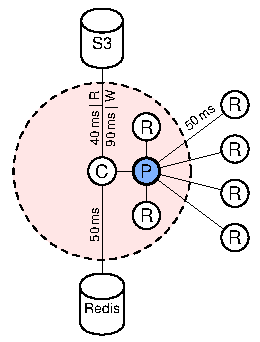
\includegraphics[width=.32\linewidth]{ps/diag-2}
        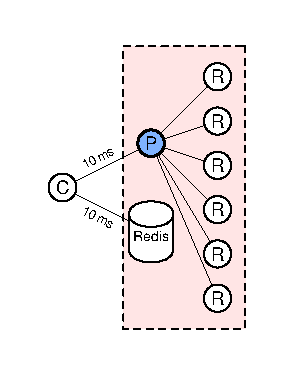
\includegraphics[width=.32\linewidth]{ps/diag-3}\\
        (a) \hspace{2.7cm} (b)
    \caption{Deployment scenarios: (a) cloud client, (b) colocation center. The shaded area represents a
    LAN (or a data center). Latencies will be used in the evaluation.
    $C$ is the client, $R$ is a replica and $P$ is the proxy replica.
    }\label{fig:deployments}
\end{figure}


To minimize the chance of correlated faults of individual metadata
servers, each replica can be at a different location, depending on the
deployment scenario. For example, the \ac{TEEMS} replicas may be
distributed over multiple administrative domains to make it less
likely that several of them can be rolled back at any given time. One
way to achieve this distribution is to colocate some replicas with a
client in a datacenter, with the remaining replicas in other
administrative domains (Figure~\ref{fig:deployments}a).  In another
example scenario, clients execute on their own premises and wish to
share data items stored in the Cloud with other clients, without
trusting the Cloud. They can use \ac{TEEMS} replicas deployed at a local
collocation center, where subsets can be physically isolated and
operated by independent providers, possibly using storage in the same
center (Figure~\ref{fig:deployments}b).

Depending on their cost and availability needs, clients may opt to
store a single copy on a single cloud storage service provider,
multiple copies on independent providers, or multiple erasure coded
fragments on independent providers. In the common case, a copy or a
small set of fragments can be efficiently retrieved from the nearest
providers.


\section{Implementation}\label{sec:teems_impl}

We implemented the \ac{TEEMS} prototype in Intel SGX (version 1),
using C++. The \ac{TEEMS} servers are implemented using a
single-threaded event loop and 6KLoC (\ac{TEEMS}). Additionally,
the client library, which interacts with the replicas and with
the untrusted storage, takes up to 5KLoC (\ac{TEEMS}). We used
Flatbuffers~\cite{flatbuffers} to define our protocol messages
and their serialization, but implemented the secure transport
between the replicas using OpenSSL~\cite{openssl}.

\new{
It is important to observe that since in \ac{TEE} replicated
systems replicas cannot generally trust clients to execute the protocol
code correctly, our prototypes implement the driver code
collocated with the replicas. This means that, for instance, a
register write request is first sent to a \ac{TEEMS} server (typically, one
collocated with the client) which acts as a proxy and runs the
two rounds of the protocol. A possible alternative would have been
to implement a \ac{TEE} library that drives the register
protocol, which all replicas would remotely attest. We chose
not to do this, since the former approach has wider applicability
(e.g., it allows clients that do not run in \ac{TEE}-enabled
platforms to interact with a \ac{TEE} replicated system).
}

\section{Evaluation}\label{sec:teems_eval}


We evaluate the \ac{TEEMS} prototype based on the \ac{RR} model
using benchmark workloads, aiming to answer the following questions:

\begin{enumerate}
    \item What is the overhead added by \ac{TEEMS} to secure a cloud storage system under different
      deployments?  (\S\ref{ssec:teems_eval_deploy})
    \item What is the performance of this system  when used to store
      metadata for a \ac{KVS} (Redis) under a benchmark
        workload (\ac{YCSB})?
      (\S\ref{ssec:ycsb})
\end{enumerate}

\paragraph{Experimental Setup.}
We ran our experiments using 7 machines  with
Intel$^\text{\textregistered}$ Xeon$^\text{\textregistered}$ E-2174G
processors running Debian Linux version 4.19 to run the replicas,
plus 2 machines equipped with Intel$^\text{\textregistered}$
Xeon$^\text{\textregistered}$ Platinum 8260M processors running Debian
Linux version 5.4: one of them to execute the clients and the other to
host Redis.
%
We again leveraged \texttt{sloth}~\cite{sloth} to simulate
different network topologies.

In our result graphs, each data point represents the median
measurement over $3,000$ requests and the error bars show the $5^{\text{th}}$ and
$95^{\text{th}}$ percentiles.

\begin{figure*}[t]
    \centering
    \begin{minipage}[t]{0.45\linewidth}
        \centering
        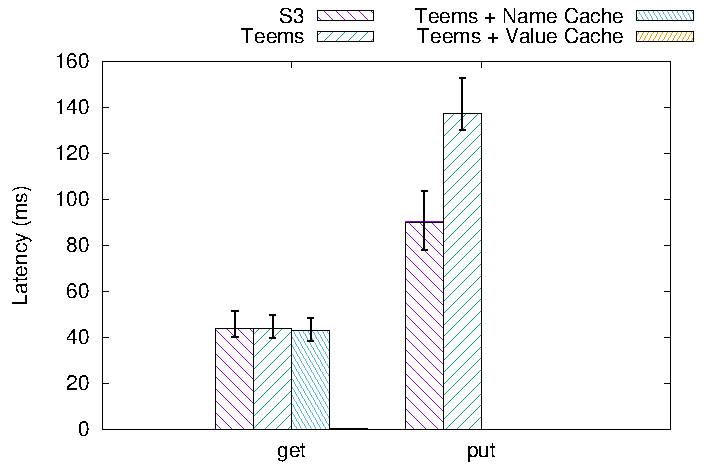
\includegraphics[width=\linewidth]{teem_results/deployment/result/client_cloud_s3}
        \caption{Client in the Cloud w/ S3}\label{fig:cloud_client_s3}
    \end{minipage}
    \begin{minipage}[t]{0.45\linewidth}
        \centering
        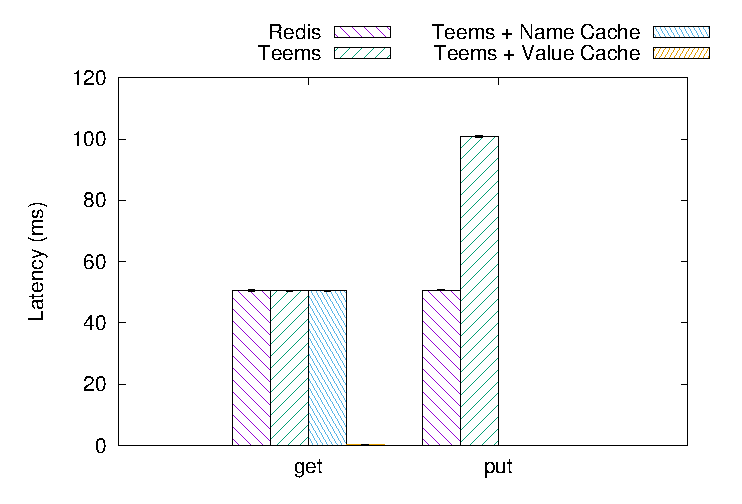
\includegraphics[width=\linewidth]{teem_results/deployment/result/client_cloud_redis}
        \caption{Client in the Cloud w/ Redis}\label{fig:cloud_client_remote_redis}
    \end{minipage}
    \begin{minipage}[t]{0.50\linewidth}
        \centering
        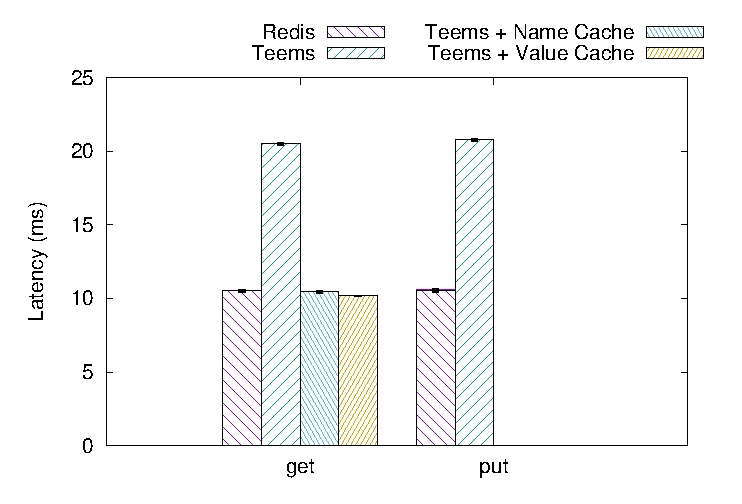
\includegraphics[width=\linewidth]{teem_results/deployment/result/collocation_center}
        \caption{Colocation Center w/ Redis}\label{fig:coloc_redis}
    \end{minipage}
    \caption{Latency in different deployment scenarios. The
    ``s3'' and ``redis'' bars refer to direct accesses to the
    untrusted storage, providing a performance baseline without
    rollback protection. ``teems'' refers to accesses without
    caching. ``teems + name cache'' and ``teems +
    blob cache'' refer to accesses where the name and blob
    caches had a hit, respectively. \new{Caching only applies for
    get requests, and in the cases of
    Figures~\ref{fig:cloud_client_s3} and~\ref{fig:cloud_client_remote_redis}
    the ``value cache'' exists, but is close to zero since the
    cache hit with a local read quorum means there is no network
    latency access in the critical path.}}
\end{figure*}



%-------------------------------------------------------------------------------
\subsection{\ac{TEEMS}-based storage}\label{ssec:teems_eval_deploy}
%-------------------------------------------------------------------------------
First, we focus on understanding the performance of our example
application, the  \ac{TEEMS}-based secure storage service, under
different deployments, which differ in the relative location of
the client, the metadata servers, and the type and location of
the untrusted storage. In this set of experiments, our baselines
are the untrusted
storage systems being used in each situation, namely Amazon S3 and an
instantiation of Redis on our local cluster, to which we optionally
add a variable  latency on the
access link.

We consider three representative deployment scenarios, illustrated in
Figure~\ref{fig:deployments}.

\paragraph{Client in the Cloud.}
In this deployment (Figure~\ref{fig:deployments}a), the client is
co-located with three metadata servers and the remaining four servers
are in another datacenter.  We use two variants of storage: a
remote Redis deployment, and S3.

\paragraph{Collocation Center.}
In this scenario (Figure~\ref{fig:deployments}b), all metadata
servers and the Redis deployment are in the same collocation center, being hosted by different cloud
providers.

In both cases, the largest administrative domain has $4$
replicas, while at most $2$ replicas are expected to crash
in a correlated fashion. As such, we consider $M_R = 4$ and $F= 2$.

From Figures~\ref{fig:cloud_client_s3}--\ref{fig:coloc_redis}, we
conclude that: 1) \ac{TEEMS} performance depends heavily on the deployment
scenario (in particular on the existence of local read quorums, which
are enabled by \ac{RR}); 2) name caching is effective at masking
the overhead of accessing the metadata store; 3) blob caching, when
combined with local read quorums, allows for local reads of both data
and metadata, outperforming the baseline.


\subsection{\ac{TEEMS}-based storage running \ac{YCSB}}\label{ssec:ycsb}

Next, we compare \ac{TEEMS} with using only
Redis, on the \ac{YCSB} benchmark workloads. We deployed \ac{TEEMS} in the
Client in the Cloud setting with Redis, using name caches. We use all six core workloads
of \ac{YCSB} (A--F), which have different key distributions and read/write
ratios. The size of the objects varies between 100B and 1KB, depending
on the workload and the overall size of the database is of
1000 1KB objects.
%
The results in Figures~\ref{fig:ycsb_teems} and~\ref{fig:ycsb_redis}
show that writes incur a $2\times$ overhead, which is expected since
the Redis access must be preceded by the \ac{TEEMS} metadata access. In
contrast, reads perform comparably to the baseline, due to local
read quorums and effective usage of the cache.

\begin{figure}[t]
    \centering
    \begin{minipage}[t]{0.49\linewidth}
        \centering
        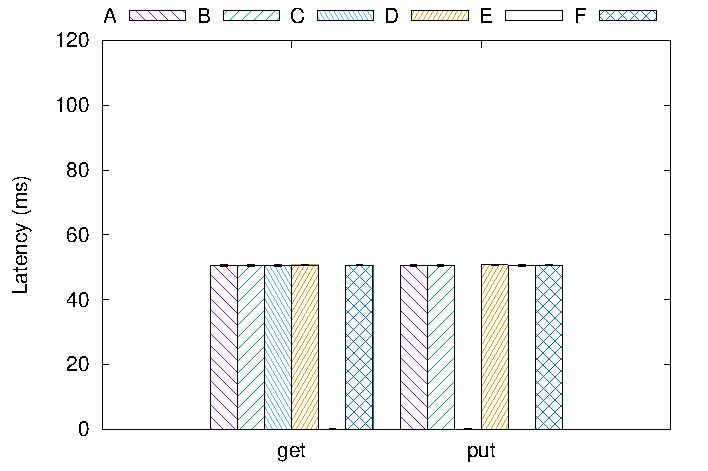
\includegraphics[width=\linewidth]{teem_results/deployment/result/ycsb_redis}
        \caption{Redis baseline}\label{fig:ycsb_redis}
    \end{minipage}
    \begin{minipage}[t]{0.49\linewidth}
        \centering
        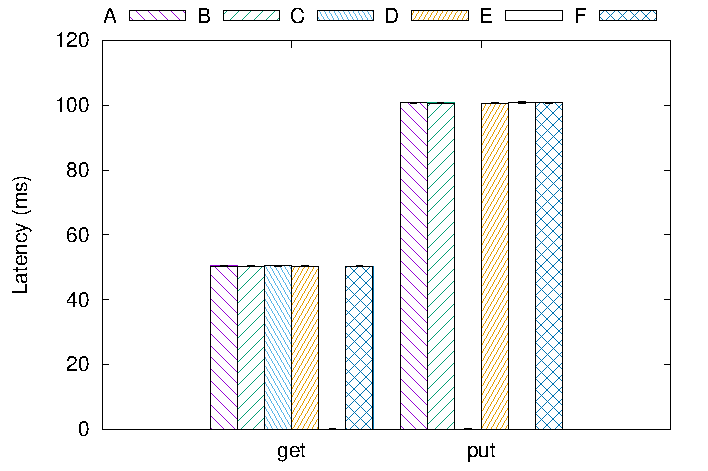
\includegraphics[width=\linewidth]{teem_results/deployment/result/ycsb_teems}
        \caption{\ac{TEEMS} + Redis}\label{fig:ycsb_teems}
    \end{minipage}
    \caption{Latency with \ac{YCSB} workloads}
\end{figure}

